\documentclass[12pt]{article}

\usepackage{sbc-template}

\usepackage{graphicx,url}
\usepackage{pifont} 
\usepackage[square,numbers]{natbib}
\usepackage[brazil]{babel}   
\usepackage{pdfpages}
\usepackage{pgfgantt}
%\usepackage[latin1]{inputenc}  
\usepackage[utf8]{inputenc}  
% UTF-8 encoding is recommended by ShareLaTex

\sloppy

\begin{document} 

\setlength{\voffset}{0cm}
\setlength{\hoffset}{0cm}

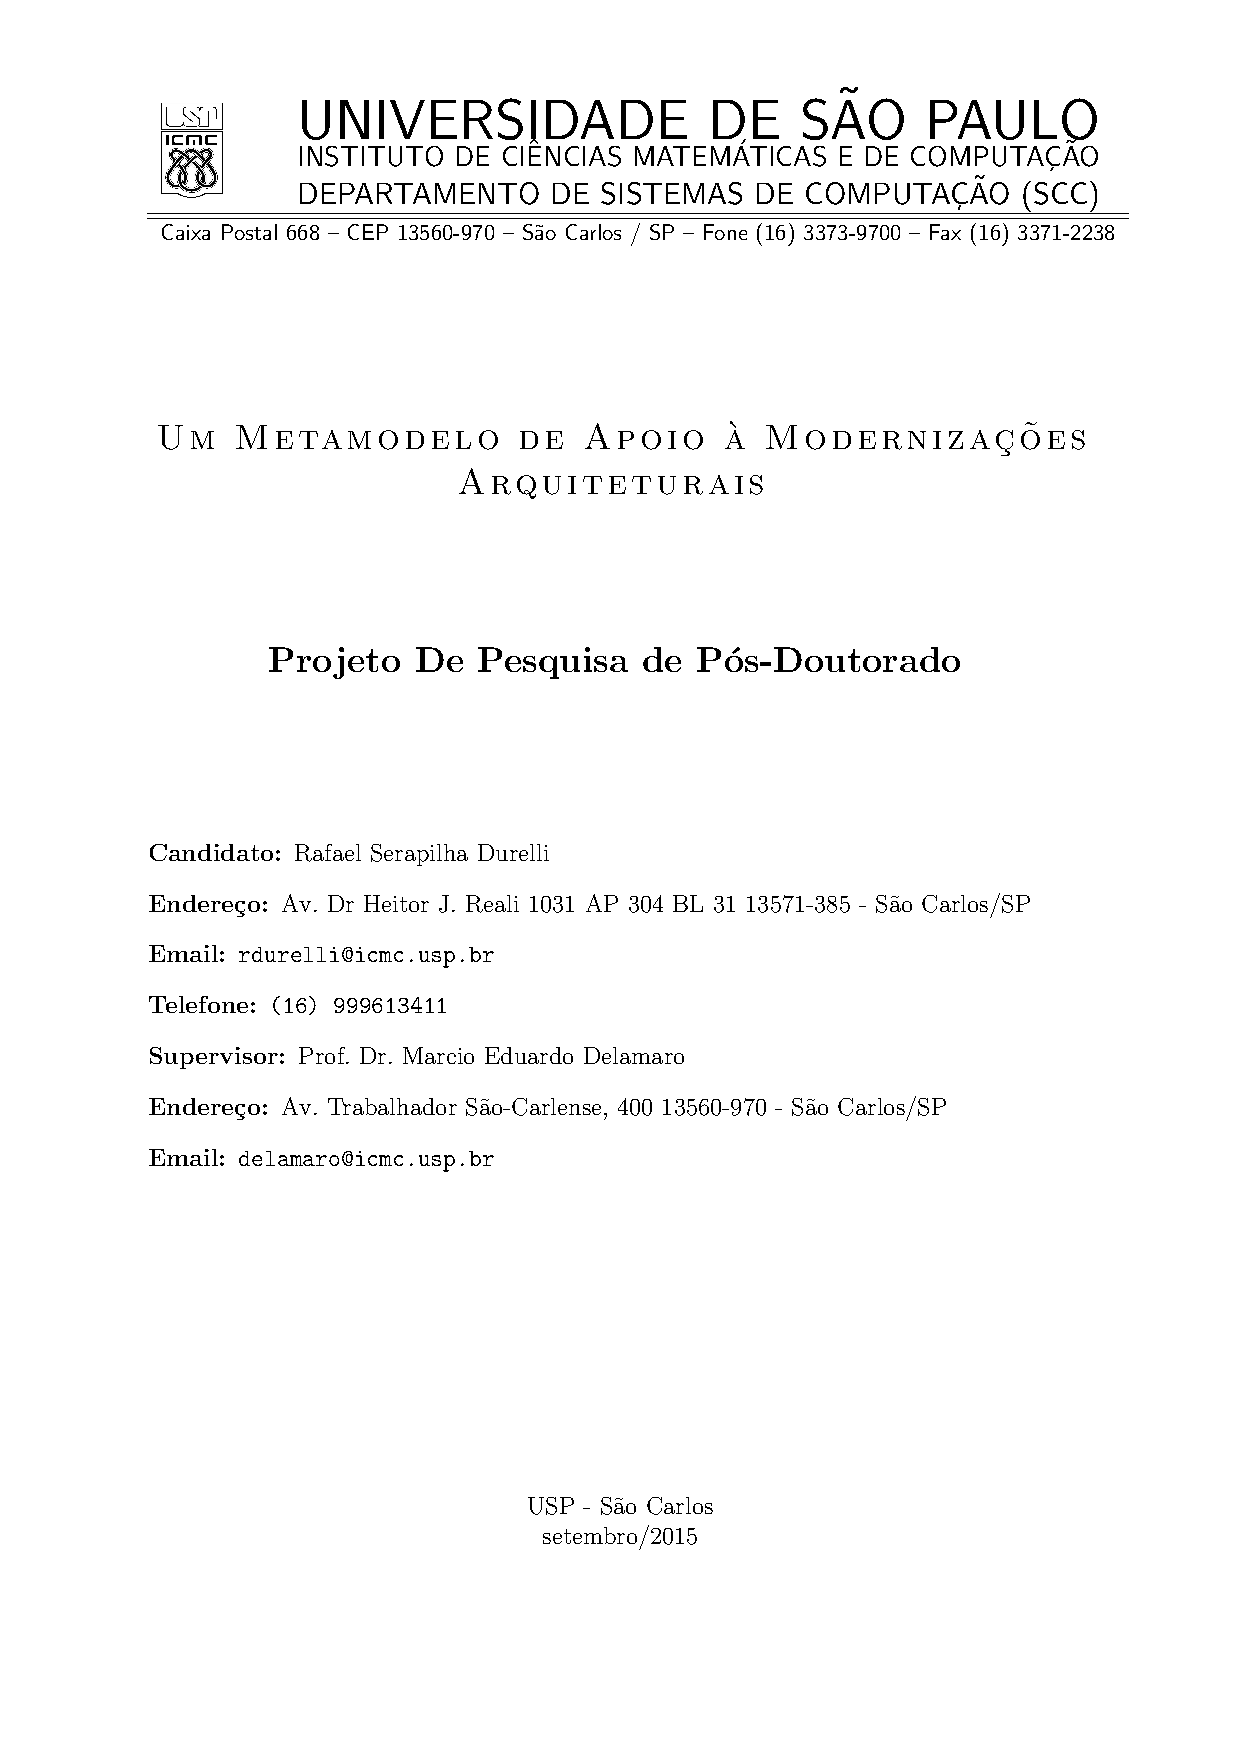
\includepdf[pages=-]{capa_pos_doutorado.pdf}

\begin{resumo}
Manter sistemas legados é uma atividade complexa e custosa para muitas empresas. Uma proposta recente para esse problema é a Modernização Dirigida à Arquitetura (\textit{Architecture-Driven Modernization} - ADM), definida pela \textit{Object Management Group} (OMG). A ADM consiste em um conjunto de princípios e metamodelos padrões que apoiam a modernização de sistemas utilizando modelos. O \textit{Knowledge Discovery Metamodel} (KDM) é o principal metamodelo da ADM, podendo representar diversos artefatos de um sistema, como código-fonte, arquitetura, interface de usuário, arquivos de configuração e processos de negócio. Embora a ADM e o KDM tenham sido criados para auxiliar o ciclo completo do processo de modernização, observa-se atualmente carência de um metamodelo que reúne as principais informações de apoio a análise de desvios arquiteturais durante os processos de modernização. A ausência de um metamodelo para apoiar a visualização de desvios arquiteturais durante o processo de modernização pode ter como resultado o aumento do esforço e consequentemente dificulta a condução adequada e efetiva de modernizações arquiteturais. Nesta perspectiva, o principal objetivo desse projeto é fazer com que modernizações arquiteturais possam ser feitas de forma mais efetiva com a ajuda de metáforas visuais. Para isso, será estabelecido um metamodelo de visualização arquitetural e também uma abordagem semiautomática  de modernização arquitetural. Assim, o engenheiro de modernização poderá visualizar e analisar falhas e desvios arquiteturais antes de efetivamente realizar a modernização do sistema. Espera-se com isso ampliar e encorar o uso a abordagem ADM, bem como seus metamodelos durante todo o processo de modernização arquitetural.
\end{resumo}

\section{Introdução}

\subsection{Contexto}

Sistemas legados são aqueles que possuem inúmeras regras de negócio de uma organização e que acomodam conhecimento de anos de manutenções. Muitos deles são ainda vitais para as organizações mas apresentam sérios problemas de manutenção. Mesmo que tenha sido construído seguindo as melhores técnicas de projeto e codificação existentes, esses sistemas tornam-se obsoletos em vistas das novas tecnologias que são disponibilizadas ou em consequência de manutenções que são feitas sem planejamento. Além das correções de erros, as mudanças mais comuns que os sistemas legados sofrem são migrações para novas arquiteturas e extensões em sua funcionalidade para atender a novos requisitos dos usuários~\cite{Krueger92, SoftwareReuse}.

Manter sistemas legados é uma atividade complexa e onerosa para muitas empresas. Uma proposta recente para esse problema é a Modernização Dirigida à Arquitetura (\textit{Architecture-Driven Modernization} - ADM), proposta pelo \textit{Object Management Group} (OMG). A ADM consiste em um conjunto de princípios e metamodelos padrões que apoiam a modernização de sistemas utilizando modelos. O \textit{Knowledge-Discovery Metamodel} (KDM) é o principal metamodelo da ADM, podendo representar diversos artefatos de um sistema, como código-fonte, arquitetura, interface de usuário, arquivos de configuração e processos de negócio. O ciclo completo de um processo de modernização na ADM se inicia com a engenharia reversa do sistema legado, prossegue com uma análise da situação atual do sistema objetivando detectar seus problemas arquiteturais, segue com reestruturações e otimizações e finaliza gerando novamente o código modernizado.


Usualmente, durante a modernização de sistemas legados o engenheiro também devera-se preocupar com a arquitetura de software desse sistema. Arquitetura de software é geralmente definida como um conjunto de decisões de projeto que tem impacto em cada aspecto da construção e evolução de sistemas de software. Isso inclui a forma como sistemas são estruturados em componentes e restrições sobre como tais componentes devem interagir. Um problema típico de sistemas legados é a erosão arquitetural. Por exemplo, a arquitetura planejada (documentação) de um sistema legado - se disponível - geralmente não reflete sua implementação atual. Na prática, desvios em relação à arquitetura planejada são comuns, devido a desconhecimento por parte dos desenvolvedores, requisitos conflitantes, dificuldades técnicas, pressões para cumprir prazos de entrega, etc. Mais importante, esses desvios arquiteturais impactam negativamente o projeto, podendo anular características essenciais de um sistema, como manutenibilidade, reusabilidade, escalabilidade e portabilidade~\cite{Passos_2010}.

Um dos mecanismo para controlar a erosão arquitetural é aplicar técnicas de Checagem de Conformidade Arquitetural (CCA). CCA é uma técnica para o controle de qualidade de software e para verificar se a implementação do sistema está de acordo com a arquitetural planejada pelos desenvolvedores~\cite{Knodel_2007}. Existem diversas técnicas para evitar a erosão arquitetural. Dentre as principais técnicas, pode-se citar: Modelos de Reflexão~\cite{Murphy_1995}, Matrizes de Dependências Estruturais~\cite{Sangal_2005}, \textit{Source Code Query Languages}~\cite{Verbaere_2008} e ArchJava~\cite{ArchJava_2202}. Após a aplicação de técnicas de CCA deve-se aplicar técnicas de reparação arquitetural para solucionar as erosões arquiteturais identificadas. Usualmente, tais reparações arquiteturais envolvem o uso de técnicas de reestruturação de software, refatoração e transformações. Dentro do ciclo típico de modernização proposto pela ADM, a CCA encontra-se logo após a engenharia reversa e antes da etapa de reestruturação. Um exemplo de abordagem ferramental que dá apoio à CCA no contexto da ADM é a ArchKDM, que foi desenvolvida pelo candidato e com colaboradores deste projeto. ArchKDM realiza CCA para identificar desvios arquiteturais utilizando como base uma instância do metamodelo KDM que representa o sistema com erosões arquiteturais. É imporante ressaltar que essa ferramenta será utilizada e possivelmente estendida para o contexto deste projeto.

Em uma linha de pesquisa paralela, encontra-se a visualização de software. Visualização de software é definida como a representação visual dos artefatos do software, tais como: requisitos, projeto e código-fonte. A principal motivação para utilizar visualização de software é para auxiliar \textit{stakeholders} a entender e compreender diferentes aspectos do software durante todo o processo de desenvolvimento/reestruturação e assim reduzir o custo da evolução do software~\cite{Diehl_2007, Gallagher_2008}. Na literatura é possível identificar algumas ferramentas que realizam a visualização de software para auxiliar durante a análise e manutenção, um exemplo desse tipo de  ferramenta é a SourceMiner~\cite{source_miner_glauco} que será utilizada no contexto deste projeto. Similarmente, técnicas de visualização também são aplicadas para a arquitetura de software. Visualização arquitetural de software é definida como a representação visual dos componentes arquiteturais. Usualmente, as arquiteturais de software são representadas em um grafo de dependência orientado, onde os vértices representam os componentes da arquitetura e as arestas representam as dependências estabelecidas entre os componentes. 

Como já salientado na literatura é possível identificar um conjunto de técnicas e ferramentas para realizar CCA~\cite{Maffort_2013, Knodel_2007, ArchJava_2202, Murphy_1995}. Porém, a grande maioria dessas técnicas e ferramentas têm como saída elementos textuais proprietários e não permitem uma análise detalhada dos desvios arquiteturais identificados. Além disso, essas ferramentas tradicionais focam apenas em realizar CCA não se preocupando com a interoperabilidade nem mesmo na representação detalhada dos desvios arquiteturais identificados~\cite{Diehl_2007, Gallagher_2008}. Uma possível solução para esse problema é a criação de um metamodelo de visualização arquitetural. Esse metamodelo reunirá um conjunto de metaclasses para representar os elementos arquiteturais, bem como desvios arquiteturais que ocorrem entre esses elementos. Esse metamodelo pode ser utilizado como base para todas as futuras e já existentes ferramentas de CCA, aumentando assim a interoperabilidade entre elas. 

É importante destacar que este projeto terá colaboração de pesquisas nacionais e internacionais entre o Instituto de Ciências Matemáticas e de Computação da Universidade de São Paulo - ICMC/USP, a Universidade de Salvador (UNIFACS) e o Institut National de Recherche en Informatique et en Automatique - INRIA/França. O candidato pretende realizar parte das atividades contidas neste plano de pós-doutorado nessas duas instituições. Dessa forma, a realização do presente projeto proporcionará um significativo incremento na formação do bolsista como pesquisador e também aumentará a qualidade das publicações científicas a serem produzidas, o que motiva sua permanência na mesma instituição em que foi conduzido seu doutorado.


\subsection{Motivação}

%Como salientado anteriormente o KDM é um metamodelo que pode ser utilizado para definir desde representações especificas de um sistema (elementos estruturais e comportamentais de código-fonte) até representações abstratas de um sistema (abstrações arquiteturais, regras de negócio, banco de dados, etc). No entanto, até o momento, existe uma carência de padronizações para auxiliar a definir como visualizar todas as representações do metamodelo KDM, ou seja, como representar visualmente todas as camadas do metamodelo KDM. Dessa forma, usualmente os desenvolvedores precisam  criar suas próprias soluções ferramentais e determinar o que, e como deverá ser visualizado no metamodelo do KDM. Como resultado, tais ferramentas tendem a diminuir a interoperabilidade e a coerência durante a visualização e apresentação de informações para os usuários dessas ferramentas. Uma definição adequada para ``visualização'' no contexto da ADM e KDM é a seguinte: ``Visualização é o processo para representar um determinado sistema como um conjunto de imagens para auxiliar na compreensão de como o sistema está implementado, com o intuito de identificar falhas e erros de projeto''~\cite{ADM:OMG}. 

No contexto deste projeto, de forma resumida pode-se especificar que as principais motivações são:

\begin{enumerate}

\item A escassez de estudos que identificam as principais metáforas visuais durante modernizações arquiteturais. Isto é, quais são as visualizações que permitem entender, analisar e resolver desvios arquiteturais de forma efetiva. A ausência de estudos desse tipo dificulta a condução adequada e efetiva de modernizações arquiteturais;

\item Ausência de um metamodelo que reúna as principais informações de apoio à análise de desvios arquiteturais em processos de modernização. A maior parte das ferramentas que permitem visualização arquitetural~\cite{Maffort_2013, Knodel_2007, ArchJava_2202} não possui foco na representação dos desvios, apenas em mostrar os elementos arquiteturais e suas relações, o que também dificulta a condução de processos desse tipo;

\item A inadequabilidade do metamodelo KDM em servir de base para a direta geração de metáforas visuais. Como esse metamodelo é direcionado à representação de artefatos de software e não de elementos gráficos, a geração de metáforas visuais a partir dele resulta em transformações excessivamente complexas e de difícil manutenção. Isso ocorre porque dentro de uma única transformação \textit{T}, haveria conhecimento relacionado a elementos de código-fonte, que precisam ser lidos do KDM, e elementos gráficos, que precisariam ser representados visualmente.
\end{enumerate}


\subsection{Objetivos}

O objetivo mais amplo deste projeto é fazer com que modernizações arquiteturais possam ser feitas de forma mais efetiva. Para que esse objetivo seja alcançado, os seguintes objetivos específicos devem ser atingidos:

\begin{enumerate}
\item Identificar metáforas visuais que fornecem apoio efetivo durante projetos de modernização arquitetural, de forma a facilitar a análise dos desvios arquiteturais de um sistema.

\item Criar um Metamodelo de Visualização Arquitetural (MVA) que reúne as metaclasses mais adequadas para a representação não só os elementos arquiteturais mas também dos desvios que ocorrem entre esses elementos. Assim como ocorre com os outros metamodelos da ADM, tal como o metamodelo SMM, o MVA que será desenvolvido neste projeto possui bastante relação com o KDM, podendo, inclusive, referenciar algumas de suas metaclasses;

\item Fazer com que as transformações de modelo tornem-se mais claras e de manutenção mais facilitada. Isso deverá ser obtido pois pretende-se dividir as transformações em dois passos: i) Transformação do KDM para MVA e depois do MVA para as metáforas visuais;

\item Estender a ferramenta SourceMiner~\cite{source_miner_glauco} com o objetivo de criar novas metáforas visuais arquiteturais para auxiliar o engenheiro de modernização durante a modernização da arquitetura de um software. Essas novas metáforas irão se concentrar em apresentar os desvios arquiteturais que o software contêm, bem como os elementos que estão violando a arquitetura; 

\item Encorajar desenvolvedores de ferramentas de modernização a utilizarem o KDM e o MVA proposto para aumentar a interoperabilidade entre as futuras e atuais ferramentas de modernização arquitetural.

\end{enumerate}


%Neste projeto de pós-doutorado, o objetivo é o desenvolvimento de uma abordagem de modernização, completa e automática, que permita visualizar o impacto positivo e negativo que determinado conjunto de transformação tem no sistema, antes de efetivamente conduzir o processo. Assim, o engenheiro poderá analisar o cenário de modernização antes de efetivamente realizar a modernização do sistema por intermédio de apoio de representações visuais.

%Para isso, inicialmente, o engenheiro de modernização deve obter um panorama dos problemas atuais do sistema, o que será feito por meio de uma nova abordagem de mineração com o foco em identificar elementos de código que implementam os conceitos da arquitetura alvo. As abordagens atuais de mineração tem enfoque na identificação de tipos específicos de interesses, não sendo eficazes na identificação de tipos variados. Dessa forma, pretende-se evoluir duas ferramentas (SourceMiner e CCKDM) já desenvolvidas por colaboradores deste projeto~\cite{source_miner_glauco, daniel_san_journal} no sentido de permitir que elas possam minerar elementos de código que implementam os conceitos arquiteturais.

%A análise da arquitetura será apoiada pelo uso combinado de um conjunto de metáforas visuais instanciadas a partir do metamodelo proposto. As metáforas poderão ser ajustadas a partir dos filtros disponíveis na interface gráfica de forma que nem todos os elementos armazenados no metamodelo sejam representados visualmente na tela. Isto possibilita a configuração do cenário visual de acordo com o objetivo da atividade de compreensão da arquitetura realizada. Por exemplo, será possível configurar os filtros para que seja dada ênfase às características de determinado modelo arquitetural alvo. Assim, será possível ajustar as metáforas visuais para indicar módulos do sistema que tenham mais coesão e menos acoplamento com outros módulos; ou se o sistema analisado está aderente a um conjunto de regras de uma determinada arquitetura ou ainda para indicar o grau de modularização de determinados interesses transversais como persistência e segurança.

%Depois do ajuste das metáforas visuais de acordo com as características esperadas para uma possível arquitetura alvo, poderá ser feita a análise do que deverá ser feito para transformar o sistema estudado. Isto será possível pelo fato de cada modelo arquitetural alvo possuir um conjunto de metáforas visuais indicado para sua representação e também um conjunto de filtros que podem ser utilizados para apoiar a análise. Isto apoiará a execução das transformações que visam a atender aos requisitos que foram especificados pelo modernizador. Os modelos arquiteturais recomendados pela abordagem poderão ser comparados quantitativamente. Desta forma, o nível de atendimento da arquitetura recomendada 1 atente a 70\% do modelo arquitetural alvo, enquanto que o modelo arquitetural recomendado 2 atende a 90\% do modelo arquitetural alvo. Depois de analisar os modelos arquiteturais, o modernizador poderá escolher pelo mais adequado e assim a abordagem irá efetivamente modernizar o sistema. 

\subsection{Experiência do Grupo com ADM e KDM}

É importante destacar que o candidato, bem como colaboradores deste projeto possuem vasta experiência em ADM e KDM. Durante o projeto de doutorado do candidato, Bolsa de Doutorado FAPESP, Processo N. 2012/05168-4, juntamente com parcerias, foram definidos e elaborados um conjunto de soluções para auxiliar e colaborar com a ADM e seus metamodelos: por exemplo, em~\cite{dani_san_tool, dani_san, daniel_san_journal} o candidato juntamente com uma parceria desenvolveram técnicas de mineração de interesse transversal com a utilização do metamodelo KDM. Em ~\cite{Santos_2014, santo_wmod} o candidato com a colaboração de outro pesquisador criaram um perfil para permitir que o metamodelo KDM desse total suporte ao Paradigma Orientado a Aspecto (POA) durante a modernização de sistemas, uma iniciativa para utilizar o metamodelo SMM também foi desenvolvida~\cite{honda_dissertacao}.  Uma ferramenta denominada ArchKDM para realizar CCA também foi desenvolvida pelo candidato e colaboradores.

Além disso, foi identificado pelo candidato uma ausência de catálogos de refatorações adaptados para o metamodelo KDM~\cite{durelli_systematic_mapping} - a vantagem seria que qualquer catálogo adaptado para o KDM seria independente de plataforma e de linguagem de programação - aumentando assim o reuso e a interoperabilidade entre diversas ferramentas de modernização. Dessa forma, o candidato desenvolveu um conjunto de refatorações e um ambiente totalmente automatizado para auxiliar a aplicação de refatorações para o metamodelo KDM~\cite{durelli_catalogo, durelli_VEM_ferramenta}. Durante um mapeamento sistemático conduzido~\cite{durelli_systematic_mapping} pôde-se observar na literatura a carência de estudos que definem soluções para especificar refatorações para o KDM. De acordo com a OMG, sem a adequada representação de refatorações no contexto do metamodelo KDM, a realização e a reutilização de uma refatoração pode se tornar uma atividade propensa a erros e difícil. Dessa forma, o candidato definiu um metamodelo para persistir metadados de refatorações, ou seja, o principal objetivo desse metamodelo é ser uma iniciativa e uma proposta para a especificação ADM \textit{Refactoring Specification} (ADMRS). Esse metamodelo permite a representação de refatorações de granularidade fina e grossa, porém, ainda respeita a independência de linguagem e plataforma uma das principais características e vantagens dos metamodelos definidos pela ADM. 

\subsection{Organização da Proposta}

O restante deste projeto está organizado da seguinte forma. Na Seção~\ref{sec:fundamentacao_teorica} a fundamentação teórica é apresentada, dando especial atenção ao metamodelo KDM e visualização de software no contexto da ADM e KDM. Na Seção~\ref{sec:proposta_de_trabalho} a proposta do projeto é apresentada. Essa seção é dividida em seis subseções (\textit{i}) Desafios de Pesquisa com Relação ao Projeto; (\textit{ii}) Plano de Trabalho e Cronograma; (\textit{iii}) Materiais e Métodos; (\textit{iv}) Contribuições e Resultados Esperados; (\textit{v}) Avaliação e Disseminação; (\textit{vi}) Resultados Relacionados. Por fim, a Seção~\ref{sec:colaboracoes} apresenta os pesquisadores que irão colaborar para a realização do projeto aqui proposto.

\section{Fundamentação Teórica}\label{sec:fundamentacao_teorica}

\subsection{\textit{Architecture-Driven Modernization} e \textit{Knowledge Discovery Metamodel}}

Em 2003 a OMG iniciou esforços no sentido de padronizar o processo de modernização de sistemas legados utilizando modelos por meio \textit{Architecture-Driven Modernization Task Force} (ADMTF). O objetivo da ADM é revitalizar os sistemas existentes melhorando ou adicionando funcionalidades, reutilizar os padrões existentes de modelagem da OMG e da iniciativa \textit{Model-Driven Architecture} (MDA) e consolidar as melhores práticas que conduzem à modernização bem sucedida. A OMG por meio da ADMTF teve a iniciativa de padronizar os processos da reengenharia de software para aumentar o êxito nos projetos dessa natureza~\cite{PerezCastillo:2011jo}. 

Para dar suporte ao processo de modernização, foi criado em 2006 um metamodelo que possibilita a comunição entre diferentes plataformas e linguagens, e foi chamada pela ADMTF de \textit{Knowledge Discovery Metamodel} (KDM). O KDM é um metamodelo de representação intermediário comum para sistemas existentes e seus ambientes operacionais. Utilizando essa representação para sistemas existentes é possível trocar representações do sistema em modelo entre plataformas e linguagens com a finalidade de analisar, padronizar e transformar os sistemas existentes~\cite{PerezCastillo:2011jo, ADMCHAPTERR}

%Fornecendo representações para o sistemas de software existentes, o KDM consiste em vários modelos arquiteturais do sistema que são definidos em diferentes camadas de abstração. Cada modelo é representado por um conjunto de modelos KDM que representam diferentes perspectivas de conhecimento sobre os artefatos dos sistemas de software existentes. 

O KDM é estruturado de forma modular, seguindo o princípio da separação de interesse, com a capacidade de representar partes heterogêneas de um sistema. A separação de interesses no contexto do metamodelo KDM são alcançadas por meio de pacotes, como apresentado na Figura~\ref{kdm:domain}. Cada pacote está em um nível de conformidade e possui o objetivo de definir um ponto de vista arquitetural do sistema. Em outras palavras, cada pacote do KDM constitui uma determinada ontologia para descrever e representar a grande maioria dos artefatos de sistemas de software existentes. Esses pacotes podem ser criados automaticamente, semiautomaticamente ou manualmente por meio da aplicação de várias técnicas de extrações de conhecimento, de análise e de transformações. 

\begin{figure}[htb]
 \centering
 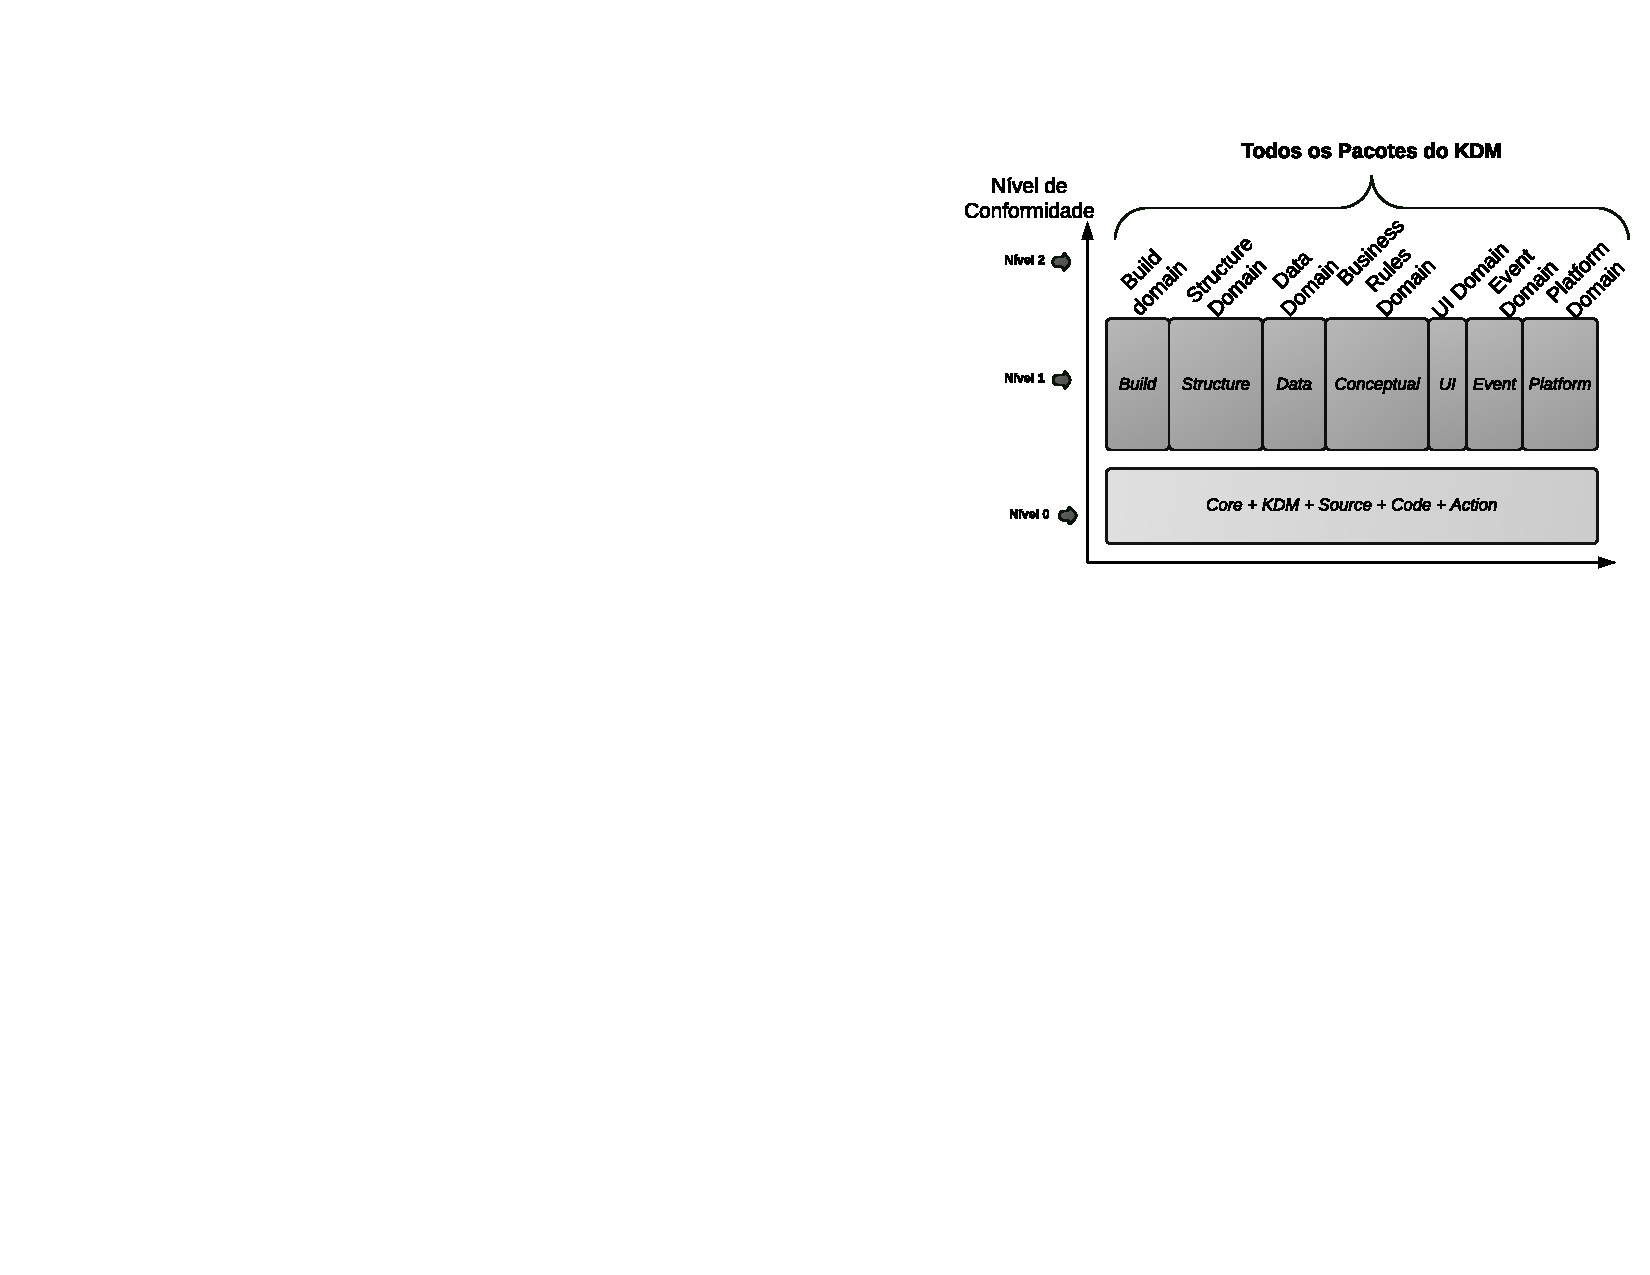
\includegraphics[scale=1]{kdmLevels_pacotes.pdf}
 \caption{Pacotes e nível de conformidade do metamodelo KDM.}
 \label{kdm:domain} 
\end{figure}

Da perspectiva de um engenheiro de software, essa separação de interesse do KDM, por meio de pacote, significa que o engenheiro só precisa se preocupar com os pacotes do KDM que considerar necessários para as suas atividades de modernização, por exemplo, uma determinada abordagem pode necessitar apenas do pacote \texttt{Code} e \texttt{Action}, enquanto uma outra abordagem utilize apenas o pacote responsável por definir elementos arquiteturais. Se essas abordagens forem evoluídas ao longo do tempo e necessitarem de outros pacotes do KDM, os respectivos pacotes podem ser adicionados ao repertório da abordagem/ferramenta, conforme necessário.

\subsection{Checagem de Conformidade Arquitetural}

Conforme um projeto de software é desenvolvido, sua arquitetura está sempre evoluindo à media que seu sistema também evolui. Portanto, são necessários meios de rastrear essas evoluções e outros aspectos implícitos do sistema de software. Esse processo é chamado  de Checagem de Conformidade Arquitetural (CCA). Torna-se, assim, imprescindível para um sistema de software garantir a conformidade entre a arquitetura planejada e sua implementação atual. A CCA é uma atividade chave para o controle de qualidade de software que têm como objetivo revelar as diferenças entre a arquitetura planejada e o código-fonte. A CCA expõe o que não esta em conformidade entre as restrições impostas na arquitetura planejada e as expressões, declarações e instruções no código-fonte~\cite{Knodel_2007}. A conformidade arquitetural pode ser verifica estaticamente, comparando o código-fonte com a visão arquitetural do sistema, ou dinamicamente, verificando o código-fonte em tempo de execução ou por meio de suas versões ao longo do tempo. Knodel e Popescu~\cite{Knodel_2007} comparam técnicas para checagem de conformidade arquitetural e citam os modelos de reflexão e as regras de relações de conformidade como duas das principais técnicas de verificação estática. 

A CCA avalia as dependências entre os componentes os resultados podem ser divididos em: (\textit{i}) \textbf{convergência}: é uma relação entre dois componentes que é permitida e foi implementada como pretendida. A convergência indica que a implementação é compatível com a arquitetura planejada; (\textit{ii}) \textbf{divergência}: é uma relação entre dois componentes que não é permitida e não foi implementada como pretendida. A divergência aponta que a implementação não é compatível com o modelo arquitetural planejado; e (\textit{iii}) \textbf{absência}: é uma relação entre dois componentes que não era pretendida, porém foi implementada. A absência indica que as relações na implementação não foram encontradas na arquitetura planejada.


Define-se como erosão arquitetural o fenômeno que ocorrer quando a arquitetura implementada de um sistema diverge de sua arquitetura planejada~\cite{Silva2012}. Existem diversas técnicas para evitar a erosão arquitetural, bem como para se realizar a CCA, pode-se citar: Modelos de Reflexão~\cite{Murphy_1995}, Matrizes de Dependências Estruturais~\cite{Sangal_2005}, \textit{Source Code Query Languages}~\cite{Verbaere_2008}, ArchJava~\cite{ArchJava_2202} e ArchKDM. Dessas técnicas a  ArchKDM foi desenvolvida pelo candidato com auxílio de colaboradores. Devido ao fato da mesma utilizar como entrada instâncias do metamodelo KDM e apresentar uma alta expressividade na forma de se tratar o problema de erosão arquitetural o candidato escolheu utilizar a ArchKDM neste projeto. É importante salientar que a maioria das técnicas disponíveis para evitar a erosão arquitetural e para realizar a CCA têm como saída elementos complexos usualmente textuais que não permitem uma fácil análise e uma verificação detalhada dos desvios arquiteturais identificados. Assim, neste projeto o candidato pretende aplicar técnicas de visualização de software para enriquecer e melhorar o entendimento dos desvios arquiteturais identificados.  

\subsection{Visualização de Software}

Os seres humanos têm a habilidade natural para controlar e detectar padrões visuais e essa capacidade pode ser explorada para melhorar a compreensão do software. A visualização é um importante meio de compreensão e é fundamental para apoiar a construção de um modelo mental ou uma imagem mental a respeito de alguma representação visual~\cite{spence2014information}. Visualizar é uma atividade cognitiva, apoiada por representações visuais externas através das quais se constrói uma representação mental interna do cenário visual observado~\cite{spence2014information, ware2012information}. No processo de visualização, dados são transformados em imagem. A imagem, por sua vez, é interpretada pelo ser humano. A interpretação de uma imagem pode conduzir à descoberta de informação a partir do que foi codificado graficamente. Isto fecha o ciclo da visualização que tem o objetivo de permitir que informação relevante seja obtida a partir de um conjunto de dados~\cite{source_miner_glauco}. 

\begin{figure}[h]
 \centering
 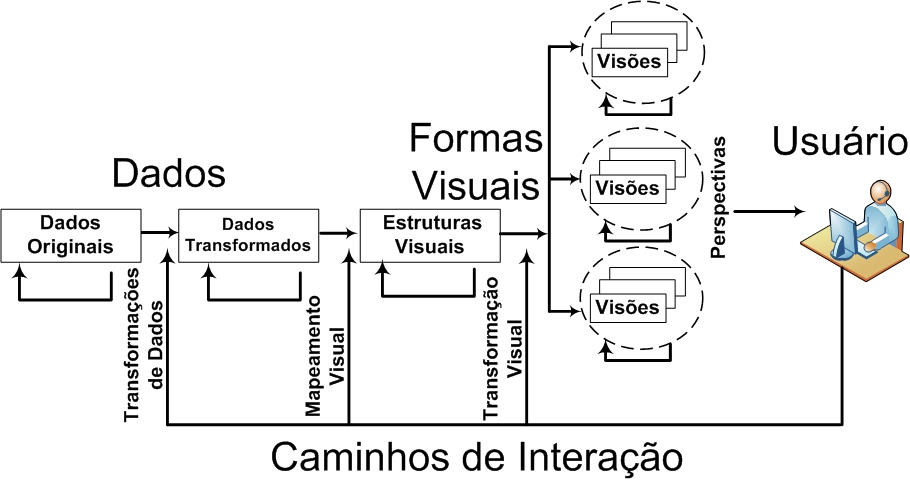
\includegraphics[scale=0.39]{image.png}
 \caption{Modelo de \textit{Card} adaptado para Múltiplas~ Visões~\cite{source_miner_glauco}.}
 \label{fig:modelo_card}
\end{figure}

Uma visão é uma representação visual de um conjunto de dados. A análise de conjuntos de dados complexos tipicamente requer múltiplas visões, cada uma revelando um aspecto diferente dos dados sob análise~\cite{Boukhelifa_2003}. Este é o caso em engenharia de software, pois uma única visão não necessariamente apoiará a compreensão efetiva dos dados nela representados~\cite{Storey_2006}. Múltiplas visões incentivam a construção de conhecimento mais aprofundado a respeito dos dados analisados e evitam interpretações distorcidas que poderiam emergir de uma única visão~\cite{Ainsworth_1999}. A Figura~\ref{fig:modelo_card} apresenta uma adaptação do modelo \textit{Card}~\cite{source_miner_glauco} para a obtenção de um modelo de referência para visualização de informações baseada em múltiplas visões. Múltiplas visões devem ser concebidas de forma consistente para que seja viável a coordenação e integração entre elas. Visões (e formas visuais) devem ser complementares entre si. Um subconjunto de visões deve ser selecionado para uso coordenado durante execução de uma determinada atividade de análise de dados~\cite{WangBaldonado_2000}. A exploração interativa das visões deve ocorrer para que sejam descobertos informações e relacionamentos que se fossem avaliados da forma tradicional permaneceriam ocultos. 

No contexto deste projeto, o conjunto de dados está relacionado à modernização arquitetural e o modelo mental construído a partir das representações de um ambiente interativo baseado em múltiplas visões. Assim, esse conjunto de dados terá o objetivo de tornar mais efetiva a análise de cenários de modernização arquitetural e consequentemente decisões mais fundamentadas nestes cenários poderão ser tomadas. Acredita-se que a definição de um metamodelo de visualização para a ADM e KDM irá beneficiar os modernizadores de software pois aumentará a interoperabilidade e a coerência durante a visualização e apresentação de informações de um determinado sistema. Além disso, esse metamodelo também auxiliará modernizadores a visualizar e entender desvios arquiteturais de forma dinâmica antes da aplicação de refatorações em sistemas que estão em conformidade ao metamodelo KDM. 

De acordo com a OMG, a ausência de uma forma bem definida para visualizar todas as visões conceituais de um sistema representado utilizando o metamodelo KDM, pode fazer com que modernizadores ignorarem ou até mesmo esquivem de problemas que precisam ser solucionados nesses sistemas. Um exemplo de ambiente que aplica os conceitos apresentados nessa seção é o SourceMiner (ver Seção~\ref{sec:source_miner})~\cite{source_miner_glauco}. A ferramenta  SourceMiner será utilizada como base para a criação e definição das metáforas arquiteturais visuais deste projeto. 

\subsection{A Ferramenta SourceMiner}\label{sec:source_miner}

Apesar dos recursos fornecidos pelos ambientes de desenvolvimento integrados modernos (do termo em inglês \textit{Integrated Development Environment}, IDE), a compreensão de programa permanece como uma tarefa não trivial. Uma iniciativa conduzida por colaboradores deste projeto é a criação da ferramenta SourceMiner~\cite{source_miner_glauco}, a qual é um ambiente de visualização de software que auxilia o engenheiro de software a visualizar e entender falhas e erros de forma dinâmica. SourceMiner foi desenvolvido como um \textit{plugin} para o IDE Eclipse e contêm dois principais módulos: (\textit{i}) \textit{Renderização e Visualização} e (\textit{ii}) Ambiente de Visualização. O primeiro módulo é responsável por renderizar todas as metáforas visuais criadas pela ferramenta SourceMiner. O segundo módulo é o \textit{kernel} da ferramenta e é responsável por extrair metadados de um projeto Java utilizando o Eclipse Java \textit{Development Tool} (JDT)\footnote{https://www.eclipse.org/jdt/}. No contexto deste projeto a ferramenta SourceMiner será estendida para que ao invés de utilizar o JDT utilize o metamodelo de visualização aqui definido, bem como o metamodelo KDM aumentando assim o nível de interoperabilidade da ferramenta. A ferramenta SourceMiner foi escolhida para ser estendida neste projeto uma vez que a mesma possui a capacidade de gerar inúmeras metáforas visuais que auxiliam o engenheiro de software durante a atividade de modernização.  

\begin{figure}[h]
 \centering
 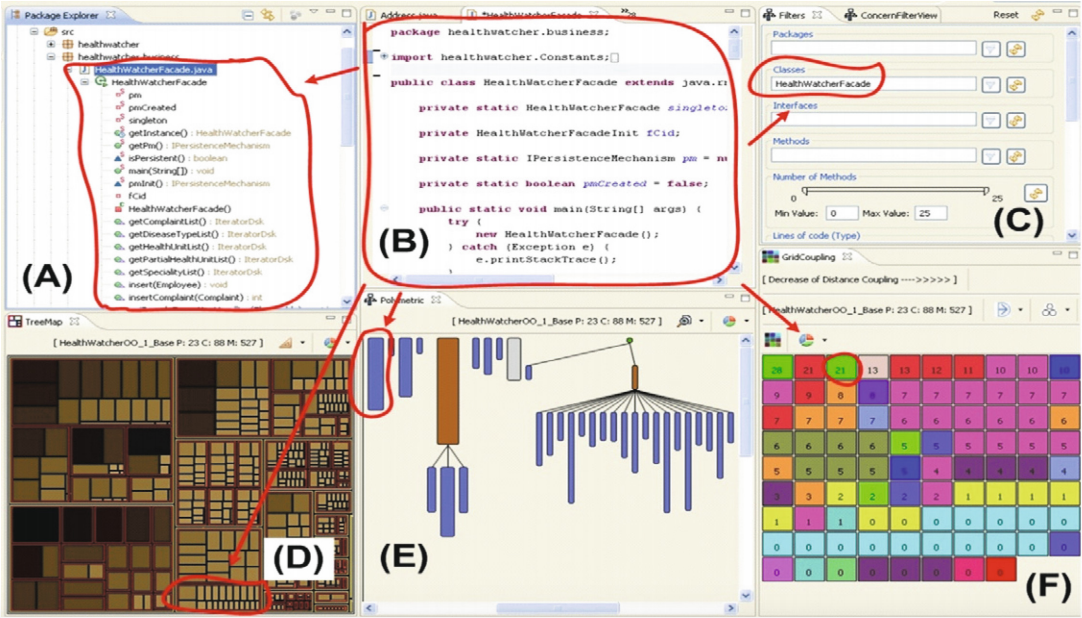
\includegraphics[scale=0.4]{sourceminerScreen.png}
 \caption{Visão Geral da SourceMiner~\cite{source_miner_glauco}.}
 \label{fig:source_miner_tool}
\end{figure}

A Figura~\ref{fig:source_miner_tool} apresenta uma captura de tela da SourceMiner. As setas indicam como uma classe específica de um sistema Java chamado \textit{HealthWatcher} é retratado em várias metáforas visuais. A parte \textbf{(B)} representa o código-fonte de uma classe aleatória do sistema \textit{HealthWatcher} e a parte \textbf{(A)} ilustra todos os pacotes e classes do sistema \textit{HealthWatcher}, ambas são visões nativas do IDE Eclipse. As partes \textbf{(D)}, \textbf{(E)} e \textbf{(F)} representam três metáforas visuais diferentes fornecidas pela SourceMiner. A parte \textbf{(D)} utiliza \textit{treemap} para representar de forma visual todos os pacotes, classes e métodos do sistema. Parte \textbf{(E)} representa uma perspectiva hierárquica de herança do projeto utilizando uma exibição polimétrica. A parte \textbf{(F)} apresenta uma perspectiva de acoplamento do sistema por meio de \textit{grid} para indicar os módulos mais acoplados do sistema. Todas as metáforas visuais apresentadas nas partes \textbf{(D)}, \textbf{(E)} e \textbf{(F)} são diretamente afetadas pela parte \textbf{(C)} que representa um filtro onde o engenheiro de modernização pode especificar o que almeja visualizar. No contexto deste projeto, esse filtro será estendido para permitir que o engenheiro de modernização possa especificar o que almeja visualizar durante a modernização arquitetural do sistema, ou seja, o engenheiro poderá especificar que almeja visualizar falhas arquiteturais, bem como visualizar quais elementos estão sendo afetados em consequência das falhas e desvios arquiteturais.

Hoje em dia a ferramenta SourceMiner não fornece nenhuma metáfora visual que apoio o processo de modernização arquitetural. Dessa forma, neste projeto também pretende-se criar novas metáforas visuais arquiteturais. Essas novas metáforas serão estudados e adaptadas na SourceMiner para auxiliar o engenheiro de modernização durante modernização da arquitetura de um software. Essas novas metáforas irão se concentrar em apresentar os desvios arquiteturais que o software contêm, bem como os elementos que estão violando a arquitetura. 

\section{Proposta de Trabalho}\label{sec:proposta_de_trabalho}

O objetivo mais amplo deste projeto é fazer com que modernizações arquiteturais possam ser feitas de forma mais efetiva. Em outras palavras, pretende-se desenvolver uma abordagem de modernização arquitetural semiautomática que permita que um engenheiro de modernização identificar, visualizar e modernizar um conjunto de desvios arquiteturais de um determinado sistema. % No contexto deste projeto, ``modelos arquiteturais alvos'' são soluções arquiteturais para serem realizadas no sistema legado que possivelmente resolverão os problemas atuais do sistema ou farão com que o sistema tenha melhores níveis de manutenibilidade, reusabilidade e extensibilidade. Exemplos de modelos arquiteturais alvos são: o padrão MVC (\textit{Model-View-Controller}), oSGI (\textit{Open Services Gateway Initiative}), camadas, componentes e SOA (\textit{Service-Oriented Architecture}).
%
Um cenário hipotético da utilização da abordagem proposta neste projeto é apresentado na Figura~\ref{fig:approach_steps} por meio da notação SADT~\cite{Marcaraf}. Os retângulos representam as atividades, as setas que entram no lado esquerdo de cada retângulo representam a entrada de dados, as setas ao lado direito representam a saída de dados. As setas no topo do retângulo representam os controles que influenciam internamente em cada atividade e as setas na base dos retângulos representam os participantes e as ferramentas utilizadas em cada atividade.

\begin{figure}[htb]
 \label{fig:approach_steps}
 \centering
 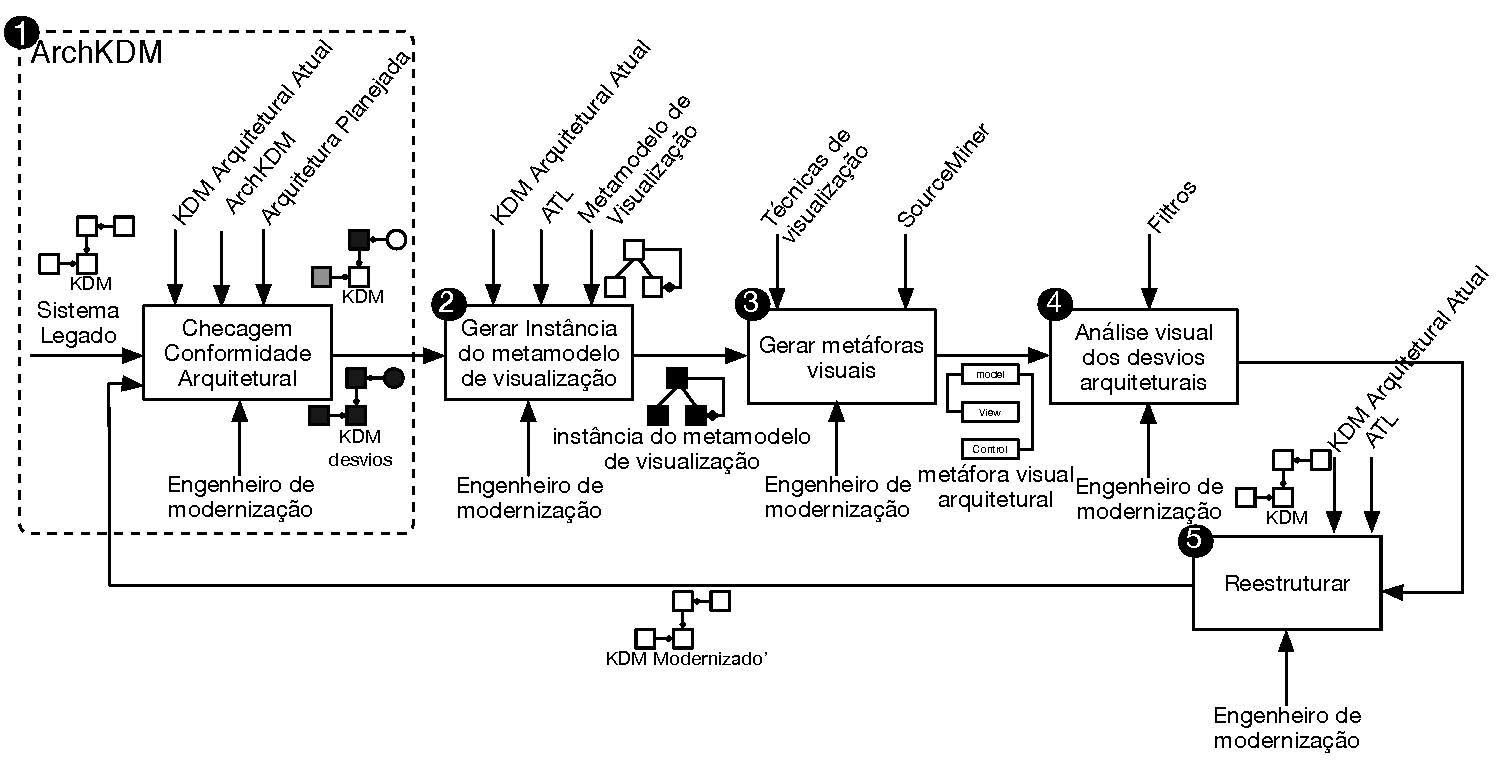
\includegraphics[scale=0.6]{projeto_pos_doc_figura6.pdf}
 \caption{Passos da Abordagem Proposta.}
\end{figure}

Antes de iniciar os passos da abordagem, primeiramente deve-se selecionar o sistema legado a ser modernizado. Em seguida, deve-se realizar a ``Checagem de Conformidade Arquitetural''. É importante evidenciar que essa atividade será realizada pela ferramenta ArchKDM, ver Figura~\ref{fig:approach_steps} \ding{182}. Essa ferramenta é capaz de identificar desvios arquiteturais tendo como entrada a instância de um sistema legado representado em KDM. Essa ferramenta já está pronta e foi desenvolvida pelo candidato juntamente com colaboradores deste projeto. Caso necessário, a mesma poderá ser estendida para satisfazer novos requisitos deste projeto~\cite{source_miner_glauco, daniel_san_journal}. 

Por meio da ArchKDM o engenheiro de modernização especifica a arquitetura planejada. Essa arquitetura deve conter os elementos arquiteturais e as restrições entre esses elementos. Os elementos arquiteturais fornecidos pela ArchKDM são: \textit{layer}, \textit{component}, \textit{subsystem}, \textit{softwareSystem} e \textit{architectureView}. Similarmente, a ArchKDM também permite especificar um conjunto de divergências (\textit{only-can}, \textit{cannot}, \textit{must}, etc) e restrições arquiteturais (\textit{access}, \textit{declare}, \textit{handle}, \textit{create}, \textit{extends}, etc). Após especificar a arquitetura planejada, a ArchKDM irá gerar como saída preliminar uma instância do metamodelo KDM que representa a arquitetura planejada do sistema.  

Em seguida, a ArchKDM gera automaticamente outra instância do metamodelo KDM que representa a arquitetura atual do sistema.  As duas instâncias do metamodelo KDM geradas (arquitetura planejada e atual) são comparadas de forma automática pela ArchKDM. Essa comparação é feita verificando os relacionamentos presentes e ausentes na arquitetura atual em relação a arquitetura planejada. Como saída, são apontados indícios de desvios arquiteturais que representam as diferenças encontradas entre as arquiteturais planejada e atual. O resultado da CCA é fornecido por meio de uma nova instância do KDM contendo todos os desvios arquiteturais identificados, ou seja, os elementos que infringiram as regras definidas na representação da arquitetura planejada do sistema legado. Uma vantagem da ArchKDM é que a mesma é uma ferramenta independente de linguagem de programação - qualquer sistema legado que seja transformado para uma instância do metamodelo KDM pode utilizar a ArchKDM.

Em sequência o segundo passo é executado, ver Figura~\ref{fig:approach_steps} \ding{183}. Esse passo utiliza como entrada uma instância do metamodelo KDM que contêm todos os desvios arquiteturais identificados no passo anterior. Em seguida essa instância é então utilizada como base para realizar a instanciação do metamodelo de visualização que será desenvolvido neste projeto. Esse metamodelo de visualização é um dos principais artefatos que será definido e criado neste projeto. Assim, maiores informações sobre o mesmo se faz necessário. Como já salientado, esse metamodelo de visualização tem como objetivo representar metadados sobre informações gráficas e visuais relacionadas a elementos e desvios arquiteturais identificados de forma dinâmica antes da aplicação de refatorações no sistema legado. 

O metamodelo de visualização a ser definido conterá metaclasses, meta-atributos e meta-relacionamentos para abstrair as metáforas arquiteturais visuais e representar desvios arquiteturais de forma independente de plataforma. O metamodelo criará e representará uma fundamentação para o compartilhamento de metadados relacionadas com metáforas arquiteturais visuais. Assim, detalhes com informações precisas sobre uma especifica metáfora visual e seus possíveis desvios arquiteturais poderão ser armazenadas e compartilhada para que outros engenheiros de modernização possam reutilizar em seus projetos. O metamodelo de visualização aqui proposto irá definir uma modelo comum para a especificação e descrição de metáforas visuais e desvios arquiteturais. Isso será alcançado por meio da padronização de modelagem \textit{Meta Object Facility} (MOF). Um dos benefícios de utilizar MOF é que o mesmo permite que o metamodelo seja serializado e deserializado sem perder nenhum tipo de informação, ou seja, instâncias do metamodelo são representadas utilizando uma representação textual padronizada XML \textit{Metadata Interchange} (XMI). Assim, o metamodelo de visualização será independente de linguagem de programação com o objetivo de fornecer uma plataforma comum pelo qual arquiteto, pesquisador e modernizador possam expressar metáforas visuais e desvios arquiteturais sem se preocuparem com a plataforma ou linguagem de programação - aumentando assim a interoperabilidade de futuras ou ferramentas existentes e técnicas de CCA.

De acordo com a OMG sem uma forma específica para visualizar os desvios arquiteturais de um sistema representado em KDM modernizadores podem ignorar problemas que precisam ser solucionados nesses sistemas. Embora o metamodelo KDM consiga representar uma grande quantidade de artefatos de um determinado sistema, o mesmo, sozinho, não é suficiente para auxiliar todo o processo de modernização arquitetural. Portanto, o metamodelo a ser definido aqui neste projeto têm como objetivo ser uma iniciativa ao pacote de visualização da ADM~\cite{ADM:visualization}.

Neste contexto, o metamodelo de visualização a ser definido neste projeto têm como objetivo ser inserido no contexto da ADM para preencher a definição de um metamodelo de visualização. Um dos objetivos desse metamodelo é seguir as padronizações propostas pela ADM. Porém, deve-se ressaltar que o metamodelo será utilizado para especificar a representação de metáforas visuais sem se preocupar com a representação das partes estruturais de uma visualização, ou seja, os elementos que serão visualizados (classes, métodos, atributos, etc.). Assim, como outros metamodelos da ADM, o metamodelo a ser definido assume que tais elementos (classes, métodos, atributos, etc.) devem ser representados utilizando outro metamodelo proposto pela ADM, como, por exemplo, o KDM. Dessa forma, o metamodelo de visualização deverá interagir com o metamodelo KDM, ou seja, o metamodelo de visualização utilizará instâncias de metaclasses do KDM. A linguagem de transformação de modelos ATL será utilizada para transformar a instância do KDM que contêm desvios arquiteturais para uma instância do metamodelo de visualização.  De forma resumida pode-se salientar que o metamodelo de visualização aqui a ser definido têm três principais objetivos: (\textit{i}) compartilhar informações sobre metáforas visuais e desvios arquiteturais; (\textit{ii}) promover o reuso de metáforas visuais; e (\textit{iii}) ser uma proposta inicial ao \textit{Call for Proposals} do ADM \textit{Visualization} da OMG. 

Após a criação da instância do metamodelo de visualização o terceiro passo (Figura~\ref{fig:approach_steps} \ding{184}) pode ser iniciado. Esse passo consiste em gerar graficamente as metáforas visuais arquiteturais do sistema. Nesse sentido, será desenvolvido um ambiente em que o engenheiro de modernização poderá visualizar um conjunto de metáforas visuais arquiteturais do sistema. Metáforas visuais que apoiam modernizações arquiteturais serão estudadas e adaptadas para este projeto. As metáforas visuais serão montadas automaticamente com base na instância do metamodelo de visualização obtida no passo anterior. Assim, o engenheiro terá a possibilidade de navegar de forma \textit{top-down} e \textit{bottom-up} (realizar \textit{zoom in} e \textit{zoom out} nos elementos arquiteturais) por essas metáforas e averiguar graficamente quais são os desvios arquiteturais que o sistema possui. Engenheiros de modernização poderão visualizar desvios arquiteturais em diversos níveis de granularidade, podendo ter uma visão ampla ou minuciosa dos problemas arquiteturais do sistema. Esse passo será apoiado pela ferramenta SourceMiner~\cite{source_miner_glauco} apresentada na Seção~\ref{sec:source_miner}, caso necessário o candidato irá estender as metáforas visuais providas pela ferramenta.


A princípio as metáforas visuais arquiteturais serão representadas por formas geométricas. Por exemplo, os pacotes serão representados por retângulos. Cada pacote conterá internamente classes que serão representadas como quadrado. Ambos os pacotes e as classes poderão ser expansíveis pelo clique do mouse - após a expansão o engenheiro de modernização visualizará os métodos em quadrados menores. As metáforas visuais também irão mostrar três tipos de dependência: (\textit{i}) dependência em nível de pacote: representará todas as dependências da arquitetura, \textit{accesses}, \textit{references}, \textit{invocations}, etc; (\textit{ii}) dependência em nível de classe: basicamente ilustrará dependência de herança entre as classes; e (\textit{iii}) dependência em nível de método: ilustrará invocações entre métodos de diferentes classes. Além dos elementos arquiteturais e suas dependências falhas também serão representadas visualmente para auxiliar o engenheiro de modernização a identificar possíveis erosões arquiteturais.


O quarto passo da abordagem é representado na Figura~\ref{fig:approach_steps} \ding{185}. Esse passo irá auxiliar o engenheiro de modernização a realizar a análise visual dos desvios arquiteturais. Essa análise da arquitetura será apoiada pelo uso combinado de um conjunto de metáforas visuais obtidas anteriormente. As metáforas poderão ser ajustadas a partir dos filtros disponíveis na interface gráfica de forma que nem todos os metadados armazenados no metamodelo de visualização sejam representados visualmente na tela. Isto possibilita a configuração do cenário visual de acordo com o objetivo da atividade de compreensão da arquitetura realizada. Por exemplo, será possível configurar os filtros para que seja dada ênfase às características de determinado modelo arquitetural. Assim, será possível ajustar as metáforas visuais para indicar módulos do sistema que tenham mais coesão e menos acoplamento com outros módulos - ou se o sistema analisado está aderente a um conjunto de regras de uma determinada arquitetura ou ainda para indicar o grau de modularização de determinados interesses transversais como persistência e segurança.

Depois que o engenheiro de modernização conduz a análise das metáforas visuais (desvios arquiteturais) poderá ser feita a reestruturação do sistema estudado no quinta passo representado na Figura~\ref{fig:approach_steps} \ding{186}. Isto será possível pelo fato de cada modelo arquitetural planejado possuir um conjunto de metáforas visuais indicado para sua representação e também um conjunto de filtros que podem ser utilizados para apoiar a reestruturação. Isto apoiará a execução das transformações que visam atender aos ``modelos arquiteturais alvos'' que foram especificados pelo modernizador. %Os modelos arquiteturais recomendados pela abordagem poderão ser comparados quantitativamente. Desta forma, o nível de atendimento da arquitetura recomendada 1 atente a 70\% do modelo arquitetural alvo, enquanto que o modelo arquitetural recomendado 2 atende a 90\% do modelo arquitetural alvo. Ainda nesse passo a abordagem irá avaliar o resultado da reestruturação do sistema com o intuito de informar ao engenheiro de modernização se a nova arquitetura atende aos requisitos informado na arquitetura planejada. Portanto, a conclusão desse passo resulta numa decisão de ``reestruturar novamente'' ou ``atende aos requisitos informado na arquitetura planejada''. Caso o novo sistema atenda aos requisitos o processo de reestruturação pode ser encerrado, caso contrário deve-se iniciar todos os passos da abordagem novamente.


\subsection{Desafios de Pesquisa com Relação ao Projeto}

Vale ressaltar que os principais desafios de pesquisa diante do projeto aqui apresentado são:

\begin{itemize}
\item Identificar quais são as informações imprescindíveis que precisam ser exibidas para apoiar decisões em processos de modernização;
\item Criar um metamodelo de visualização para aumentar a interoperabilidade e facilitar a troca de metadados sobre  metáforas visuais e desvios arquiteturais;
\item Averiguar quais são as melhores metáforas visuais que podem ser utilizadas para auxiliar efetivamente o engenheiro de modernização durante a modernização arquitetural; 
\item Estabelecer um conjunto de possíveis transformações a serem feitas durante o passo de modernização tendo como base os desvios arquiteturais identificados;
\item Desenvolver um ambiente computacional para auxiliar a aplicação da abordagem aqui proposta. Embora existem ferramentas que auxiliem a modernização de sistemas legados, existe uma ausência de ferramentas que permitam visualizar a arquitetura de um sistema, bem como seus desvios arquiteturais e permita aplicar um conjunto de transformações para modernizar o sistema.

\end{itemize}

\subsection{Plano de Trabalho e Cronograma}

Nesta seção, são listadas as principais atividades previstas para a condução deste trabalho. Na Figura~\ref{fig:gant} é apresentado o cronograma para essas atividades. Note que o cronograma é dividido em três principais etapas, as quais são comentadas a seguir:

\begin{enumerate}
\item Etapa 1: Obter conhecimento para a condução do projeto;
    
    \begin{enumerate}
    \item Pesquisa bibliográfica;
    \item Revisão ou mapeamento sistemático;
    \item Análise de técnicas de visualização;
    \end{enumerate}

\item Etapa 2: Desenvolvimento do projeto proposto e início da avaliação;

    \begin{enumerate}
    \item Identificar quais são as informações imprescindíveis que precisam ser exibidas para apoiar decisões em processos de modernização;
    \item Proposição de um metamodelo de visualização;
    \item Elaborar transformações que serão aplicadas nos sistemas legado;
    \item Desenvolvimento de uma ferramenta para dar suporte ao metamodelo de visualização;
    \item Estudo de caso da abordagem proposta;
    \end{enumerate}
    
\item Etapa 3: Avaliação e Investigação da aplicação da abordagem;

    \begin{enumerate}
    \item Avaliação experimental da abordagem proposta;
    \item Investigação de cenários práticos de aplicação da abordagem proposta.
    \end{enumerate}

\end{enumerate}

\begin{figure}[ftbp]
\begin{center}

\begin{ganttchart}[y unit title=0.5cm,
y unit chart=0.5cm,
vgrid,hgrid,
title label anchor/.style={below=-1.6ex},
title left shift=.05,
title right shift=-.05,
title height=1,
bar/.style={fill=gray!50},
incomplete/.style={fill=white},
progress label text={},
bar height=0.7,
group right shift=0,
group top shift=.6,
group height=.2]{1}{24}
\gantttitle{Cronograma de Atividades}{24} \\
\gantttitle{2016}{12} 
\gantttitle{2017}{12} \\
\gantttitle{1-Tri}{3} 
\gantttitle{2-Tri}{3} 
\gantttitle{3-Tri}{3} 
\gantttitle{4-Tri}{3}
\gantttitle{1-Tri}{3}
\gantttitle{2-Tri}{3} 
\gantttitle{3-Tri}{3} 
\gantttitle{4-Tri}{3} \\ 

%\ganttgroup{Revisão Bibliográfica}{1}{3} \\
\ganttgroup{Etapa 1}{1}{6} \\
\ganttbar{Atividade 1}{1}{1} \\
\ganttbar{Atividade 2}{2}{3} \\
\ganttmilestone{Publicar}{3} \\
\ganttbar{Atividade 3}{4}{6} \\
%\ganttmilestone{Publicar}{6} \\
\ganttgroup{Etapa 2}{4}{12} \\
\ganttbar{Atividade 4}{4}{8}\\
\ganttbar{Atividade 5}{6}{9}\\
%\ganttmilestone{Publicar}{9} \\
\ganttbar{Atividade 6}{6}{11}\\
\ganttbar{Atividade 7}{9}{12}\\
\ganttbar{Atividade 8}{10}{12}\\
\ganttmilestone{Publicar}{12} \\
\ganttgroup{Etapa 3}{13}{24} \\
\ganttbar{Atividade 9}{13}{21}\\
\ganttmilestone{Publicar}{21} \\
\ganttbar{Atividade 10}{22}{23}\\
\ganttmilestone{Publicar}{23}
%\ganttlink{elem0}{elem1}
\ganttlink{elem1}{elem2}
\ganttlink{elem2}{elem3}
\ganttlink{elem3}{elem4}
\ganttlink{elem4}{elem5}
\ganttlink{elem6}{elem7}
\ganttlink{elem7}{elem8}
\ganttlink{elem8}{elem9}
\ganttlink{elem9}{elem10}
\ganttlink{elem10}{elem11}
\ganttlink{elem11}{elem12}
\ganttlink{elem13}{elem14}
\ganttlink{elem14}{elem15}
\ganttlink{elem15}{elem16}
\end{ganttchart}
\end{center}
\caption{Cronograma\label{fig:gant}}
\end{figure}

O projeto está previsto para 2 anos, conforme ilustra a Figura~\ref{fig:gant}. As atividades 3 e 4 serão realizadas inicialmente em paralelo, pois a ferramenta será implementada à medida que as estratégias são definidas. Dessa forma, o \textit{feedback} da implementação pode contribuir para o refinamento e evolução da abordagem. Após o termino de cada etapa ou de uma macro atividade, artigos serão elaborados como apresentado na Figura~\ref{fig:gant}. 
Destaca-se que parte das atividades serão desenvolvidas junto às instituições estrangeira e nacionais vinculadas ao projeto. Planeja-se, para isso, realizar dois estágios trimestrais de pesquisa em períodos ainda a definir. 

\subsection{Materiais e Métodos}

Para as atividades de revisão bibliográfica e estudo da literatura (Atividades 1 e 2), serão empregadas técnicas de revisão sistemática e/ou mapeamento sistemático, para assegurar a validade das conclusões que podem ser extraídas dos estudos, reduzir os riscos de que esta revisão deixe de incluir estudos relevantes, além de deixar explícita quais foram as bases científicas consideradas.

Na atividade 3 serão feitas análises e discussões de possíveis técnicas de visualização que efetivamente irão auxiliar o engenheiro de modernização durante a modernização de sistemas legados. Estudos de casos serão utilizados para testar a abrangência e validade de cada técnica de visualização. Na atividade 4 pretende-se identificar quais são as informações imprescindíveis que precisam ser exibidas para apoiar decisões em processos de modernização. Para isso será investigado o nível de abstração mais adequado para auxiliar o engenheiro durante a modernização arquitetural. O objetivo é identificar termos, abstrações e metáforas visuais que são usuais em ambientes de modernização arquitetural para facilitar todo o processo de modernização.

Em seguida, na atividade 5 pretende-se criar o metamodelo padronizado de visualização. Protótipos e estudos de casos também serão realizados para testar e validar esse metamodelo. Tecnologias como o \textit{Eclipse Modeling Framework} (EMF) e \textit{Graphical Modeling Framework} (GMF) serão utilizadas nesta atividade. Na atividade 6 serão desenvolvidos algoritmos de recomendações e transformações arquiteturais. Esses algoritmos e transformações devem possuir como entrada os requisitos especificados na linguagem específica de domínio, bem como uma instância do metamodelo KDM representado o sistema legado. Tecnologias como ATL (\textit{ATL Transformation Language}) e OCL (\textit{Object Constraint Language}) serão utilizadas nesta atividade. Posteriormente, será realizado o desenvolvimento de uma ferramenta para dar total suporte a modernização. Por fim, será verificado a efetividade da abordagem por meio de experimentos. 

\subsection{Contribuições e Resultados Esperados}\label{sec:resultados_esperados}

Como principais resultados esperados com a condução das atividades que constam neste plano de trabalho, esperam-se:

\begin{enumerate}
\item Uma abordagem semiautomática  para auxiliar a atividade de modernização arquitetural de sistemas legados;
\item Evolução da atividade de modernização com o intuito de torna-lá mais sistemática e controlada;
\item Um apoio computacional para auxiliar o engenheiro durante a atividade de modernização de forma eficiente;
\item Contribuição para o grupo de Engenharia de Software do ICMC/USP, por meio do apoio em trabalhos de mestrado e doutorado relacionados ao projeto de modernização de sistemas por meio da ADM e KDM e também do apoio na orientação de projetos de iniciação científica; e
\item Relatórios técnicos e artigos publicados em conferências e periódicos nacionais e internacionais relevantes da área.
\end{enumerate}

\subsection{Avaliação e Disseminação}

Para avaliar a abordagem aqui proposta pretende-se realizar dois tipos de experimentos: (\textit{i}) estudo de caso para investigar a viabilidade da abordagem aqui proposta, bem como avaliar o uso das funcionalidades do apoio computacional para fornecer suporte a modernização arquitetural de sistemas legados; e (\textit{ii}) avaliação controlada utilizando a metodologia experimental~\cite{Wohlin}, a fim de avaliar o impacto da abordagem proposta e do apoio computacional relacionado a eficiência e impacto das equipes e também a qualidade em termos de modularidade, reuso e manutenibilidade dos sistemas resultantes durante a atividade de modernização.

Além das avaliações, os resultados alcançados serão submetidos a conferências e revistas reconhecidas. Além de uma forma de disseminação, a submissão de artigos contribuirá para a avaliação da pesquisa. Dentre as conferências de interesse, estão aquelas na área de Engenharia de Software (por exemplo, ICSE e CBSoft), bem como revistas na área de Engenharia de Software (por exemplo, JSS, STVR, TSE e TOSEM).

\subsection{Resultados Relacionados}

É importante enfatizar que apesar deste projeto de pós-doutoramento estar vinculado à mesma instituição onde o candidato realizou seu doutoramento, acredita-se que os resultados, descritos na Seção~\ref{sec:resultados_esperados}, serão alcançados de forma satisfatória. A parceria entre o candidato e o supervisor vem produzindo bons resultados, boa parte deles em cooperação com outros pesquisadores brasileiros e estrangeiros. Até o momento 22 publicações foram produzidas, a saber:

\begin{itemize}
	
	\item \textbf{2 trabalhos completos publicado como capítulo de livro}
		\begin{enumerate}
			
			\item Viana, Matheus ; Penteado, Rosângela ; Prado, Antônio do ; \textbf{Durelli, Rafael} . Developing Frameworks from Extended Feature Models. Advances in Intelligent Systems and Computing. 1ed.: Springer International Publishing, 2014, v. 263, p. 263-284.
			\item Júnior, Paulo Afonso Parreira ; Penteado, Rosângela Dellosso ; Viana, Matheus Carvalho ; \textbf{Durelli, Rafael Serapilha} ; DE CAMARGO, VALTER VIEIRA ; Costa, Heitor Augustus Xavier . Reengineering of Object-Oriented Software into Aspect-Oriented Ones Supported by Class Models. Lecture Notes in Business Information Processing. 1ed.: Springer International Publishing, 2014, v. 190, p. 296-313.
			
		\end{enumerate}
	
	\item \textbf{2 trabalhos completos publicados em revistas}
		\begin{enumerate}
			\item GOTTARDI, THIAGO ; \textbf{DURELLI, RAFAEL} ; LÓPEZ, ÓSCAR ; DE CAMARGO, VALTER . Model-based reuse for crosscutting frameworks: assessing reuse and maintenance effort. Journal of Software Engineering Research and Development, v. 1, p. 4, 2013.
			\item SANTIBÁÑEZ, DANIEL S. M. ; \textbf{DURELLI, RAFAEL} ; DE CAMARGO, VALTER . A Combined Approach for Concern Identification in KDM models. Journal of the Brazilian Computer Society, v. 1, p. 4, 2015.
		\end{enumerate}
	\item \textbf{18 trabalhos completos publicados em anais de congressos/\textit{workshops}}
	\begin{enumerate}
	    
	    \item \textbf{DURELLI, R. S.}; DURELLI, V. H. S. . A Systematic Mapping Study on Formal Methods Applied to Crosscutting Concerns Mining. In: IX Experimental Software Engineering Latin American Workshop (ESELAW), 2012, Buenos Aires. IX Experimental Software Engineering Latin American Workshop (ESELAW), 2012.
	 	
	 	\item \textbf{DURELLI, R. S.}; DURELLI, V. H. S. . F2MoC: A Preliminary Product Line DSL for Mobile Robots. In: Simpósio Brasileiro de Sistemas de Informação (SBSI), 2012, São Paulo. Simpósio Brasileiro de Sistemas de Informação (SBSI), 2012.
	 	
	 	\item Gottardi; \textbf{DURELLI, R. S.} ; PASTOR, O. L. ; CAMARGO, V. V. . Model-Based Reuse for Crosscutting Frameworks: Assessing Reuse and Maintainability Effort. In: Simpósio Brasileiro de Engenharia de Software, 2012, Natal. Simpósio Brasileiro de Engenharia de Software, 2012.
	 	\item \textbf{DURELLI, R. S.} ; Gottardi ; CAMARGO, V. V. . CrossFIRE: An Infrastructure for Storing Crosscutting Framework Families and Supporting their Model-Based Reuse. In: XXVI Simpósio Brasileiro de Engenharia de Software - XXVI Sessão de Ferramenta, 2012, Natal. Simpósio Brasileiro de Engenharia de Software, 2012. v. 6. p. 1-6.
	 	
	 	\item \textbf{DURELLI, R. S.}; SANTIBANEZ, D. S. M. ; ANQUETIL, N. ; DELAMARO, M. E. ; CAMARGO, V. V. . A Systematic Review on Mining Techniques for Crosscutting Concerns (to appear). In: ACM SAC 2013, 2012, Coimbra. ACM SAC Software Engineering (SE) Track, 2013. v. 28th.
	
	 	\item PARREIRA JUNIOR, P. A.; VIANA, M. C. ; \textbf{DURELLI, R. S.} ; CAMARGO, V. V. ; COSTA, H. A. X. ; PENTEADO, R. A. D. . Concern-Based Refactorings Supported by Class Models to Reengineer Object-Oriented Software into Aspect-Oriented Ones. In: International Conference on Enterprise Information Systems (ICEIS), 2013, ANGERS/FR. XV International Conference on Enterprise Information Systems, 2013.
		
		\item VIANA, M. C. ; \textbf{DURELLI, R. S.} ; PENTEADO, R. A. D. ; PRADO, A. F. . F3: From features to frameworks.. In: International Conference on Enterprise Information Systems (ICEIS), 2013, ANGERS/FR. XV International Conference on Enterprise Information Systems, 2013..
		
		\item VIANA, M. C. ; PENTEADO, R. A. D. ; PRADO, A. F. ; \textbf{DURELLI, R. S}. . An Approach to Develop Frameworks from Feature Models. In: International Conference on Information Reuse and Integration, 2013, San Francisco. An Approach to Develop Frameworks from Feature Models, 2013.
		
		\item VIANA, M. C. ; PENTEADO, R. A. D. ; PRADO, A. F. ; \textbf{DURELLI, RAFAEL S}. . F3T: From Features to Frameworks Tool. In: XXVII Simpósio Brasileiro de Engenharia de Software (SBES 2013), 2013, Brasília. F3T: From Features to Frameworks Tool, 2013.
		
		\item SANTIBÁÑEZ, DANIEL S. M. ; \textbf{DURELLI, RAFAEL S.} ; CAMARGO, V. V. . CCKDM - A Concern Mining Tool for Assisting in the Architecture-Driven Modernization Process. In: XXVII Simpósio Brasileiro de Engenharia de Software - XXVII Sessão de Ferramenta, 2013, Brasilia. Simpósio Brasileiro de Engenharia de Software, 2013.
		
		\item SANTIBANEZ, D. S. M. ; \textbf{DURELLI, RAFAEL S.} ; CAMARGO, V. V. . A Combined Approach for Concern Identification in KDM models. In: Latin American Workshop on Aspect-Oriented Software Development (LA-WASP), 2013, Brasília. Congresso Brasileiro de Software: Teoria e Prática (CBSoft), 2013.
		
		\item PINTO, Victor Hugo S. C. ; \textbf{DURELLI, R. S.} ; OLIVEIRA, A. L. ; CAMARGO, V. V. . Evaluating the Effort for Modularizing Multiple-Domain Frameworks towards Framework Product Lines with Aspect-Oriented Programming and Model-Driven Development. In: International Conference on Enterprise Information Systems (ICEIS), 2014, Lisboa. International Conference on Enterprise Information Systems (ICEIS), 2014.
		
		\item DIAS, D. R. C. ; \textbf{DURELLI, R. S.} ; BREGA, J. R. F. ; GNECCO, B. B ; TREVELIN, L. C. ; GUIMARAES, M. P. . Data Network in Development of 3D Collaborative Virtual Environments: A Systematic Review. In: The 14th International Conference on Computational Science and Applications (ICCSA 2014), 2014, Guimarães. The 14th International Conference on Computational Science and Applications (ICCSA 2014), 2014.
		
		\item \textbf{DURELLI, R. S.} ; SANTIBANEZ, D. S. M. ; DELAMARO, MÁRCIO E. ; CAMARGO, V. V. . Towards a Refactoring Catalogue for Knowledge Discovery Metamodel. In: IEEE International Conference on Information Reuse and Integration, 2014, San Francisco. IEEE International Conference on Information Reuse and Integration, 2014. p. 1-8.
		
		\item \textbf{DURELLI, R. S.} ; SANTIBANEZ, D. S. M. ; MARINHO, B. S. ; HONDA, R. R. ; DELAMARO, M. E. ; ANQUETIL, N. ; CAMARGO, V. V. . A Mapping Study on Architecture-Driven Modernization. In: IEEE International Conference on Information Reuse and Integration, 2014, San Francisco. IEEE International Conference on Information Reuse and Integration, 2014. p. 1-8.
		
		\item MARINHO, B. S. ; CAMARGO, V. V. ; HONDA, R. R. ; \textbf{DURELLI, R. S.} . KDM-AO: An Aspect-Oriented Extension of the Knowledge Discovery Metamodel. In: 28th Brazilian Symposium on Software Engineering (SBES), 2014, Maceió. 28th Brazilian Symposium on Software Engineering (SBES), 2014. p. 1-10.
		
		\item MARINHO, B. S. ; \textbf{DURELLI, RAFAEL S.} ; HONDA, R. R. ; CAMARGO, V. V. . Investigating Lightweight and Heavyweight KDM Extensions for Aspect-Oriented Modernization. In: 11th Workshop on Software Modularity (WMod) -- Brazilian Conference on Software: theory and practice, 2014, maceio. 11th Workshop on Software Modularity (WMod) -- Brazilian Conference on Software: theory and practice, 2014.
		
		\item \textbf{DURELLI, RAFAEL S.} ; MARINHO, B. S. ; HONDA, R. R. ; DELAMARO, MÁRCIO E. ; CAMARGO, V. V. . KDM-RE: A Model-Driven Refactoring Tool for KDM.. In: II Workshop on Software Visualization, Evolution and Maintenance -- Brazilian Conference on Software: theory and practice, 2014, Maceio. II Workshop on Software Visualization, Evolution and Maintenance -- Brazilian Conference on Software: theory and practice, 2014. p. 1-8.

\end{enumerate}
\end{itemize}

Além dessas publicações, outros artigos estão submetidos ou em fase final de escrita. É importante destacar que o candidato contará com a infraestrutura já existente no ICMC-USP, bem como a interação com outros alunos de mestrado e doutorado que já trabalham com Engenharia de Software, ADM, KDM e técnicas de visualização. Existe ainda a possibilidade de coorientação de alunos de iniciação científica e de mestrado.

\section{Colaborações}\label{sec:colaboracoes}

O presente projeto será executado em colaboração com o grupo de engenharia de software da Universidade Federal de São Carlos (UFSCar), Universidade de Salvador (UNIFACS) e o \textit{Institut National de Recherche en Informatique et en Automatique} - INRIA/França. Na UFSCar o candidato contará com o apoio e suporte do Prof. Dr. Valter Vieira de Camargo\footnote{http://buscatextual.cnpq.br/buscatextual/visualizacv.do?id=S819089}, o qual tem grande experiência na área de engenharia de software com ênfase em desenvolvimento de \textit{frameworks} no contexto da programação orientada a aspectos, reuso de software e no desenvolvimento de abordagens que utilizam ADM e KDM. Na UNIFACS, o candidato irá trabalhar juntamente com o Prof. Dr. Glauco de Figueiredo Carneiro\footnote{http://buscatextual.cnpq.br/buscatextual/visualizacv.do?id=K4799340J3} o qual possui grande conhecimento em técnicas de visualização para auxiliar todo o processo de engenharia de software. No INRIA, o candidato irá trabalhar em colaboração com o o pesquisador Nicolas Anquetil\footnote{http://rmod.inria.fr/web/team/nicolas-anquetil}, que tem grande experiência na área de engenharia de software e \textit{model-driven development}.

\small
\bibliographystyle{unsrt}
\bibliography{sbc-template}

\end{document}